\section{Metodología y Propuesta de Solución}

\subsection{Propuesta de Solución}
La propuesta de solución consiste en el diseño e implementación de un modelo predictivo global basado en una arquitectura Transformer, el cual es pre-entrenado mediante un enfoque \textit{Cross-Site Learning} sobre un conglomerado de plantas solares consolidadas. El propósito central es transferir este conocimiento climático hacia instalaciones nuevas que sufren de escasez de datos e intermitencias operativas (\textit{Cold-Start}), logrando proyecciones estables desde sus primeros días de conexión a la red.

Con base en los requerimientos técnicos de integridad informativa, el alcance empírico abarca instalaciones solares consolidadas y agrupadas estratégicamente por Macrozona. En lugar de limitar la muestra a un número fijo de plantas en una única región, el enfoque \textit{Cross-Site} capitaliza la diversidad geográfica y climática disponible, empleando algoritmos de imputación robustos para aquellos vacíos operativos manejables. Esta configuración garantiza que el modelo asimile una correlación termodinámica auténtica y representativa, permitiendo transferir el aprendizaje a nuevas instalaciones independientemente de su ubicación, siempre que compartan el perfil macrozonal.
Desde la perspectiva algorítmica, el proyecto adopta la arquitectura \textit{Temporal Fusion Transformer} (TFT) debido a su capacidad innata para procesar de forma asimétrica datos multimodales: asimilando variables dinámicas meteorológicas temporales en conjunto con características estáticas geográficas. Para dictaminar la efectividad de esta red frente a la problemática de arranque en frío, se contrastará su rendimiento de extrapolación (\textit{Zero-Shot}) frente a otras arquitecturas globales de \textit{Deep Learning} (\textit{Informer} y \textit{N-HiTS}, junto a un \textit{XGBoost} global) y contra líneas base estrictamente locales (\textit{XGBoost}, \textit{LSTM} y \textit{N-HiTS} entrenadas de forma aislada por planta), conformando un total de ocho configuraciones evaluadas bajo un protocolo idéntico.

\begin{figure}[htbp]
  \centering
  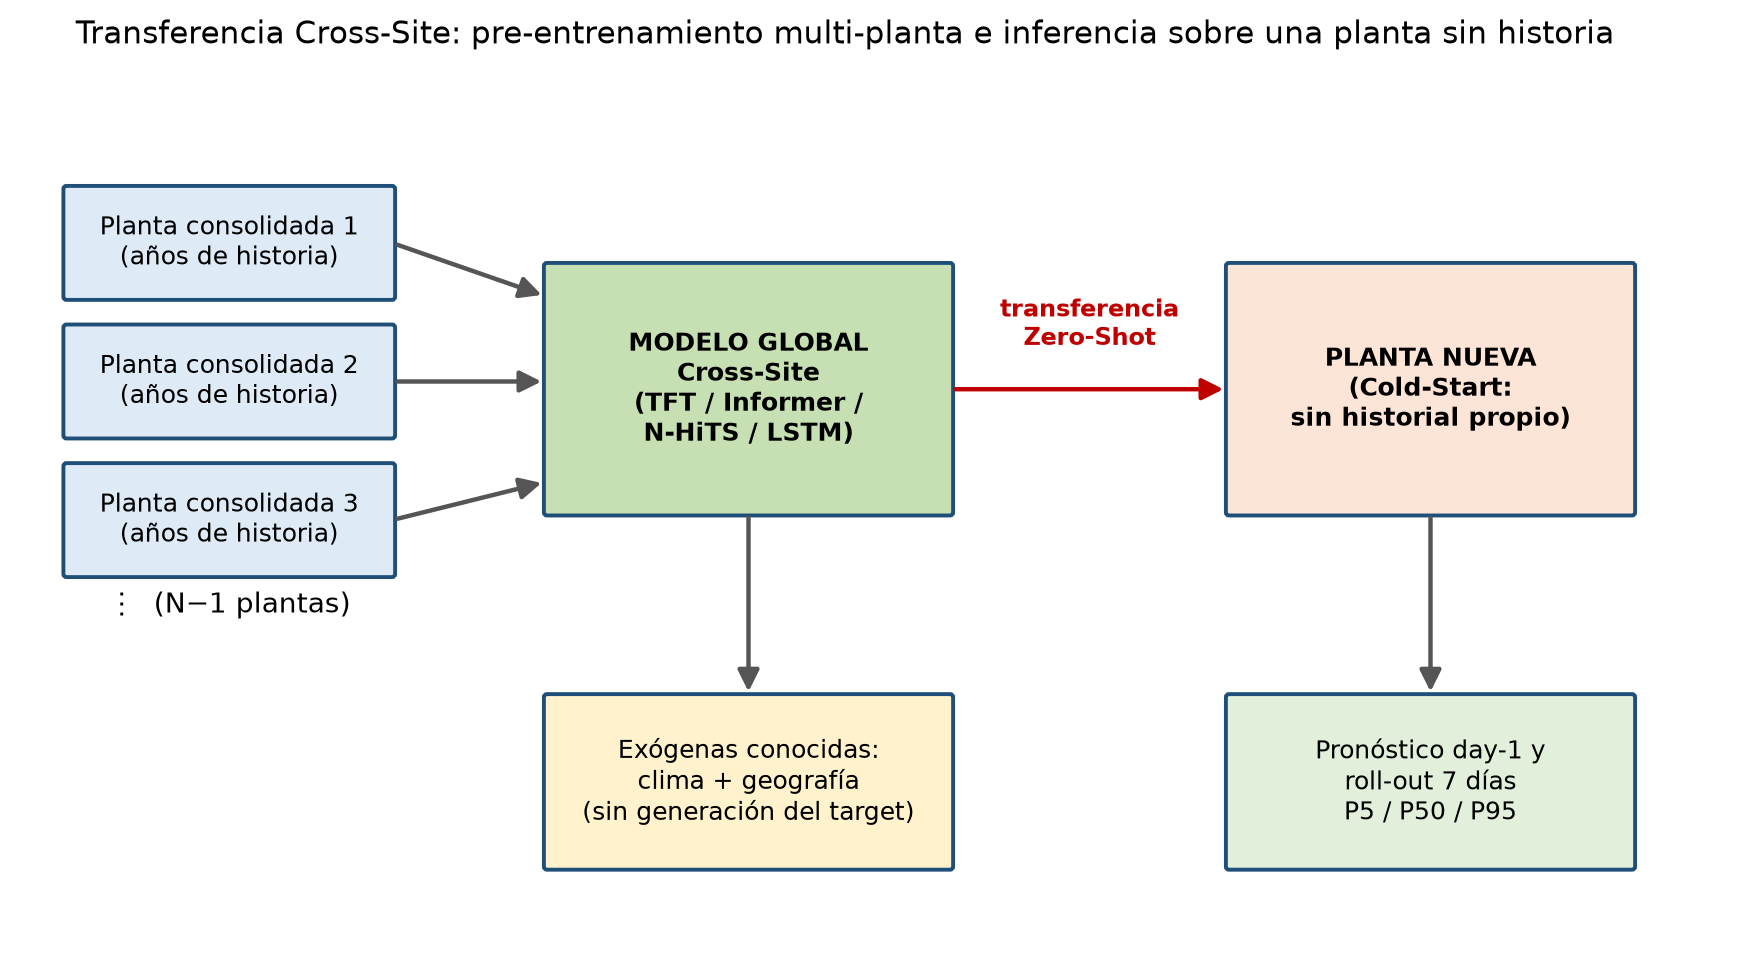
\includegraphics[width=\textwidth]{figuras/fig_solucion.png}
  \caption{\label{fig:diagrama_solucion} Representación esquemática de la propuesta de solución predictiva.}
\end{figure}

\subsection{\label{p:adaptacion}Adaptación Metodológica (Pipeline de Trabajo)}
Para sistematizar la ejecución del proyecto y asegurar la replicabilidad de los experimentos, la investigación se apoya en un \textit{pipeline} de \textit{Machine Learning Operations} (MLOps) segmentado en cuatro fases metodológicas secuenciales implementadas en lenguaje Python.

\subsubsection{Fase 0: Extracción, Transformación y Carga (ETL)}
La fase fundacional del orquestador aborda el acondicionamiento integral de los datos estructurando el proceso en un modelo de capas secuenciales \textit{Medallion} (Landing, Bronze, Silver y Gold). Para mitigar los cortes de sensores y evitar el \textit{Data Leakage}, se definieron reglas estrictas:
\begin{enumerate}
    \item \textbf{Variables Exógenas y Agrupación:} La imputación de variables meteorológicas se realiza escalonadamente (interpolación lineal y \textit{ffill}/\textit{bfill} por grupos temporales), y se incorpora una variable indicadora booleana (\textit{dummy}) para señalar registros imputados. Además, se aplican características cíclicas (\textit{seno/coseno}) para capturar estacionalidad y se impone un forzamiento a cero en la irradiancia global durante períodos nocturnos garantizados.
    \item \textbf{Manejo Estricto del Target (Intocable):} A diferencia de las variables exógenas, la variable objetivo (generación de energía) no es sometida a ningún tipo de imputación ni se rellena con ceros lógicos. Si un registro horario está ausente, permanece como NaN en el vector final. Los modelos administran estas intermitencias mediante la reindexación de la grilla horaria, y las métricas penalizan exclusivamente sobre observaciones reales y existentes. Esta decisión asegura que el \textit{Performance Ratio} no se distorsione sintéticamente.
\end{enumerate}

\begin{figure}[htbp]
  \centering
  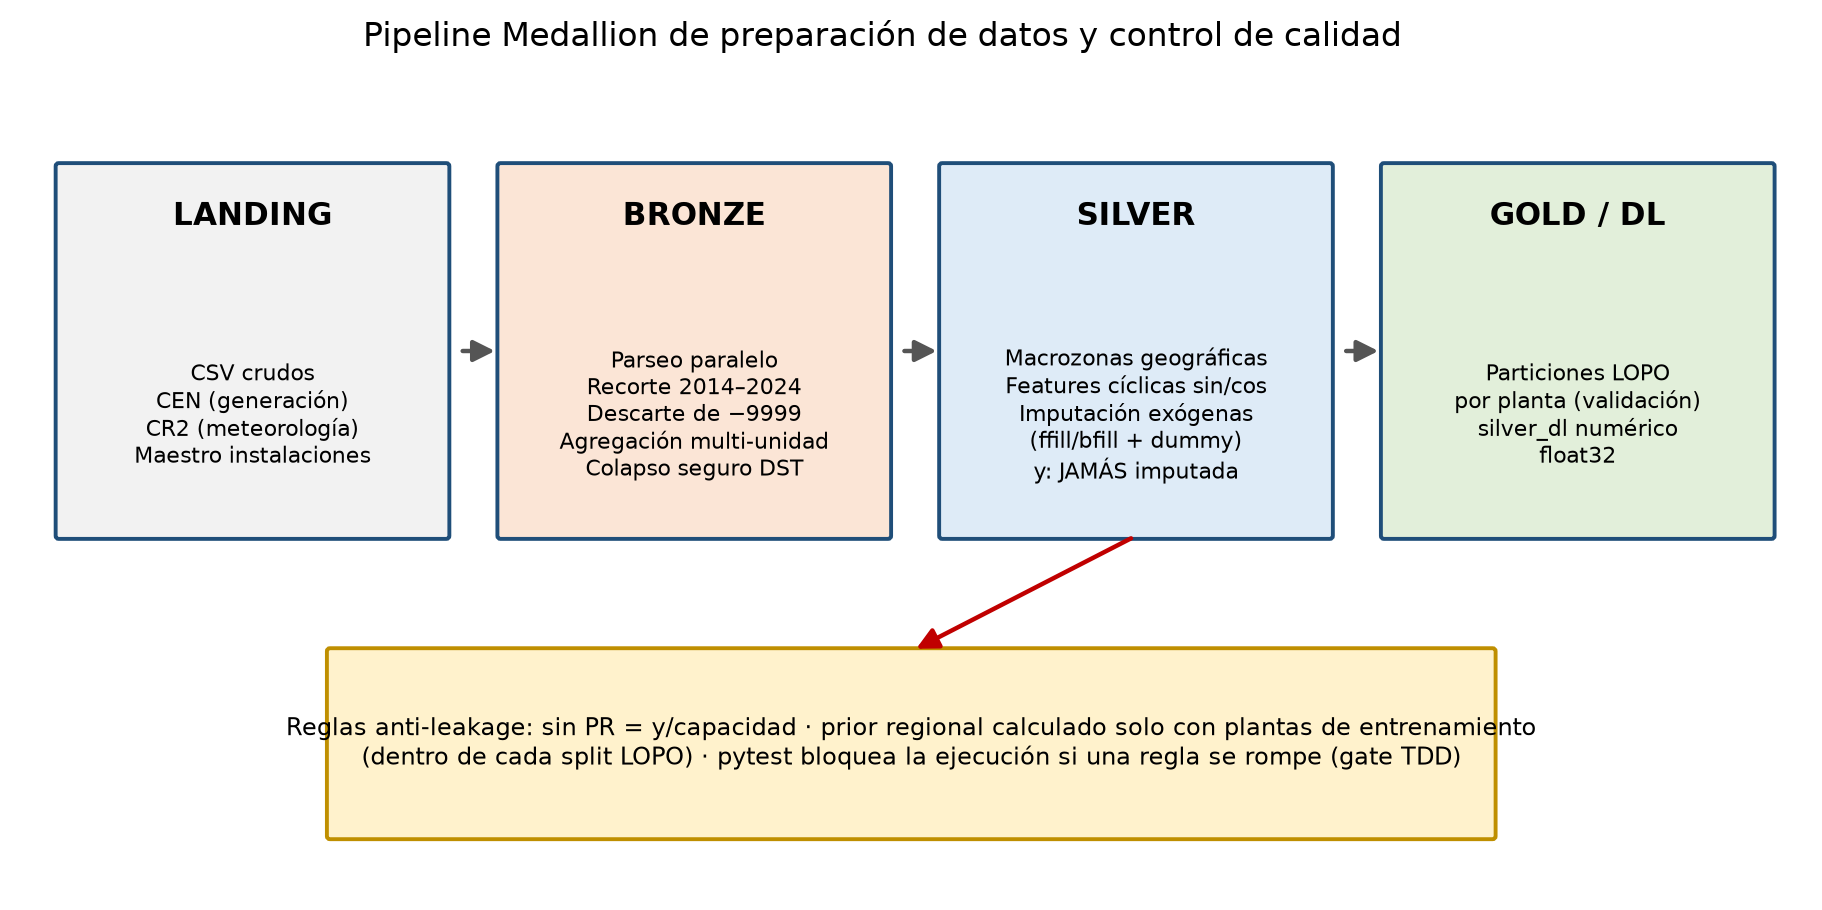
\includegraphics[width=\textwidth]{figuras/fig_etl_flow.png}
  \caption{\label{fig:etl_flow} Algoritmia del proceso de preparación de datos y control de calidad.}
\end{figure}

\subsubsection{Fase 1: Sintonización de Hiperparámetros (Tuning)}
Para garantizar una comparativa justa (\textit{Benchmarking}) entre las redes profundas globales y los algoritmos tradicionales locales, es imperativo descubrir la configuración óptima de la topología de las redes. En esta etapa, el orquestador emplea heurísticas de búsqueda y validación cruzada para sintonizar los hiperparámetros críticos (tasa de aprendizaje, profundidad del codificador, número de cabezales de atención en el TFT y tamaño de la ventana temporal) maximizando el rendimiento predictivo inicial sobre el corpus histórico general antes de someter a los modelos al estrés del arranque en frío.

\subsubsection{Fase 2: Simulación Cold-Start (Estrategia LOPO)}
El núcleo de la experimentación reside en la aplicación de la metodología de retención espacial \textit{Leave-One-Plant-Out} (LOPO). En lugar de dividir el set de datos cronológicamente, el orquestador aísla dinámicamente y oculta por completo el historial operativo de una de las plantas (capa \textit{Gold} de validación). 
El modelo \textit{Cross-Site} es entrenado exclusivamente con los años de experiencia del resto de la flota operativa. Para emular el arranque en frío (\textit{Cold-Start}) de la planta seleccionada, el contexto histórico (\textit{seed}) previo al horizonte de pronóstico se inicializa de forma 100\% sintética ($y = \text{capacidad} \times \text{PR regional} \times \text{perfil solar}$), garantizando así que no exista \textit{Data Leakage}. Dicho coeficiente de \textit{Performance Ratio (PR) regional} se calcula como un agrupamiento histórico estratificado por Macrozona y Estación del Año, computado empleando única y estrictamente el conjunto de entrenamiento. Una vez consolidados los pesos sinápticos, la red es forzada a inferir el comportamiento energético futuro de la planta oculta utilizando únicamente sus coordenadas estáticas y el clima entrante. Este procedimiento se repite iterativamente rotando la instalación objetivo. Asimismo, la orquestación de esta fase admite la ejecución bajo distintas escalas (\textit{Toy}, \textit{Half} y \textit{Total}) que modulan la fracción de la muestra analizada, agilizando el \textit{benchmarking}.

\begin{figure}[htbp]
  \centering
  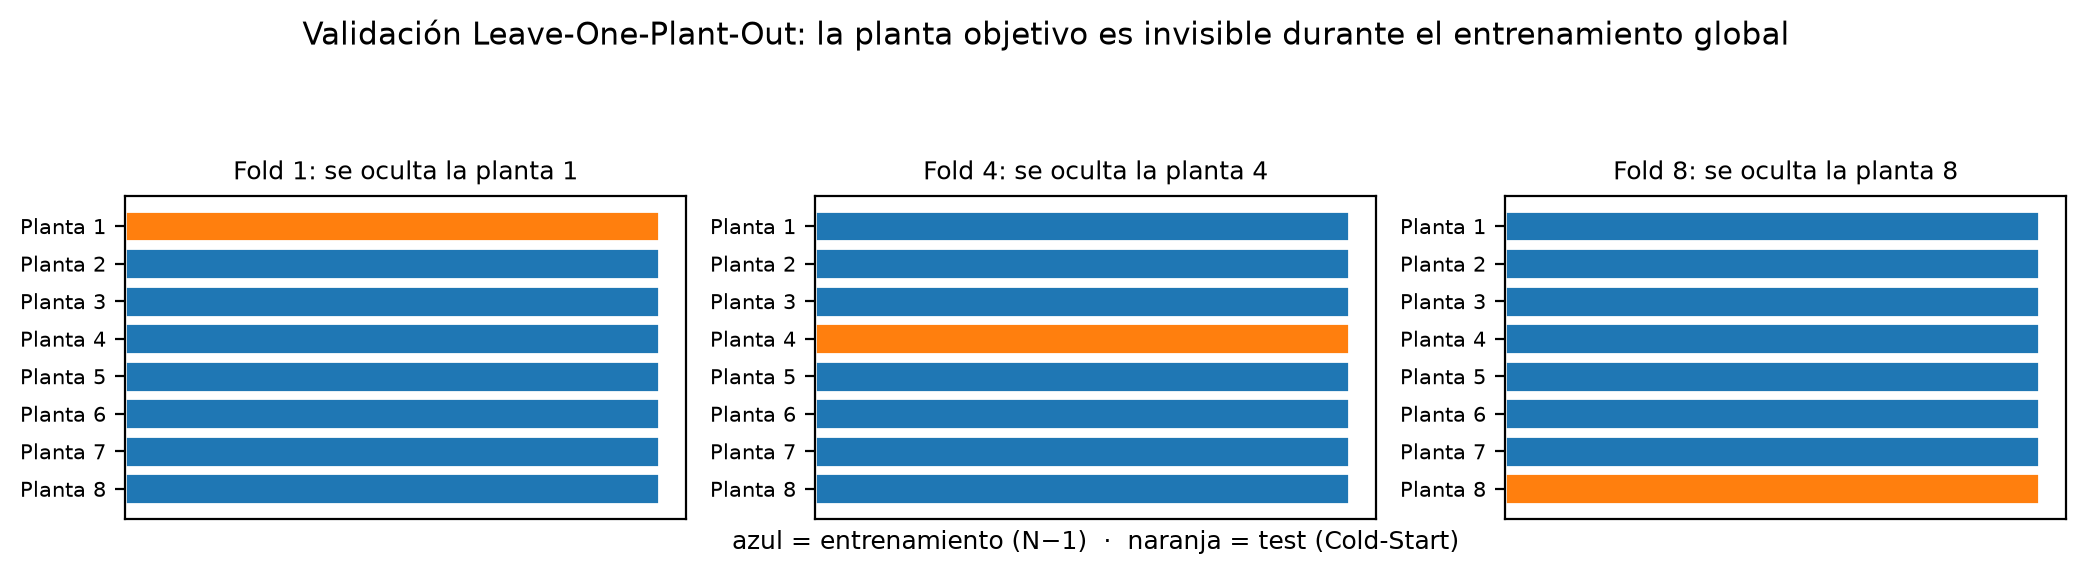
\includegraphics[width=\textwidth]{figuras/fig_lopo.png}
  \caption{\label{fig:lopo_strategy} Visualización iterativa del aislamiento espacial para simulación de arranque en frío.}
\end{figure}

\subsubsection{Fase 3: Extracción de Resultados y Métricas de Rendimiento}
La fase final consolida los vectores predictivos generados por cada una de las arquitecturas sometidas a prueba —modelos globales \textit{Cross-Site} (TFT, Informer, N-HiTS, LSTM y XGBoost Global) y líneas base estrictamente locales entrenadas con la historia propia de cada planta (XGBoost, LSTM y N-HiTS locales)— contrastándolos unificadamente contra la producción energética empírica de los parques solares aplicando 2 estrategias de testeo diferenciadas según la ventana temporal proyectada (\textit{day1} para predicción a 24 horas y \textit{rollout7d} para proyección expandida iterativa a una semana).
Adicionalmente, los resultados y desvíos son evaluados de manera estratificada según la \textbf{Estación del Año}, lo que permite medir el impacto de la variabilidad meteorológica cíclica en las redes. El proyecto computa métricas clásicas de pronóstico, entre las cuales destacan:
\begin{itemize}
    \item \textbf{Error Absoluto Medio (MAE):} Para cuantificar la magnitud promedio lineal del error en la escala energética real (MW).
    \item \textbf{Error Cuadrático Medio (RMSE):} Para penalizar cuadráticamente las desviaciones más grandes generadas por los sesgos del modelo durante picos de inyección, dado que eleva al cuadrado cada error antes de promediarlo.
    \item \textbf{Error Porcentual Absoluto Medio Simétrico (sMAPE):} Empleado como estándar de industria para dimensionar la falla en términos relativos porcentuales, independientemente de la capacidad instalada de la planta.
    \item \textbf{Pronóstico Probabilístico:} los modelos emiten intervalos de predicción del 90\,\% (cuantiles P5/P50/P95) para reportar la incertidumbre esperada. Su calidad se evalúa mediante dos indicadores distintos: la \textbf{cobertura empírica}, definida como la frecuencia con que la observación real cae dentro del intervalo (idealmente cercana al 90\,\% nominal), y la \textbf{pérdida pinball} (\textit{pinball loss}), una función de costo cuantílica que penaliza de forma asimétrica los errores por encima y por debajo de cada cuantil. Las predicciones finales se ajustan para cumplir leyes físicas (mínimo de cero general y cero estricto de noche).
\end{itemize}
La consolidación de estas métricas se tabulará y graficará para facilitar el análisis comparativo financiero y operativo entre el modelo Transformer global y las líneas base locales.

\begin{figure}[htbp]
  \centering
  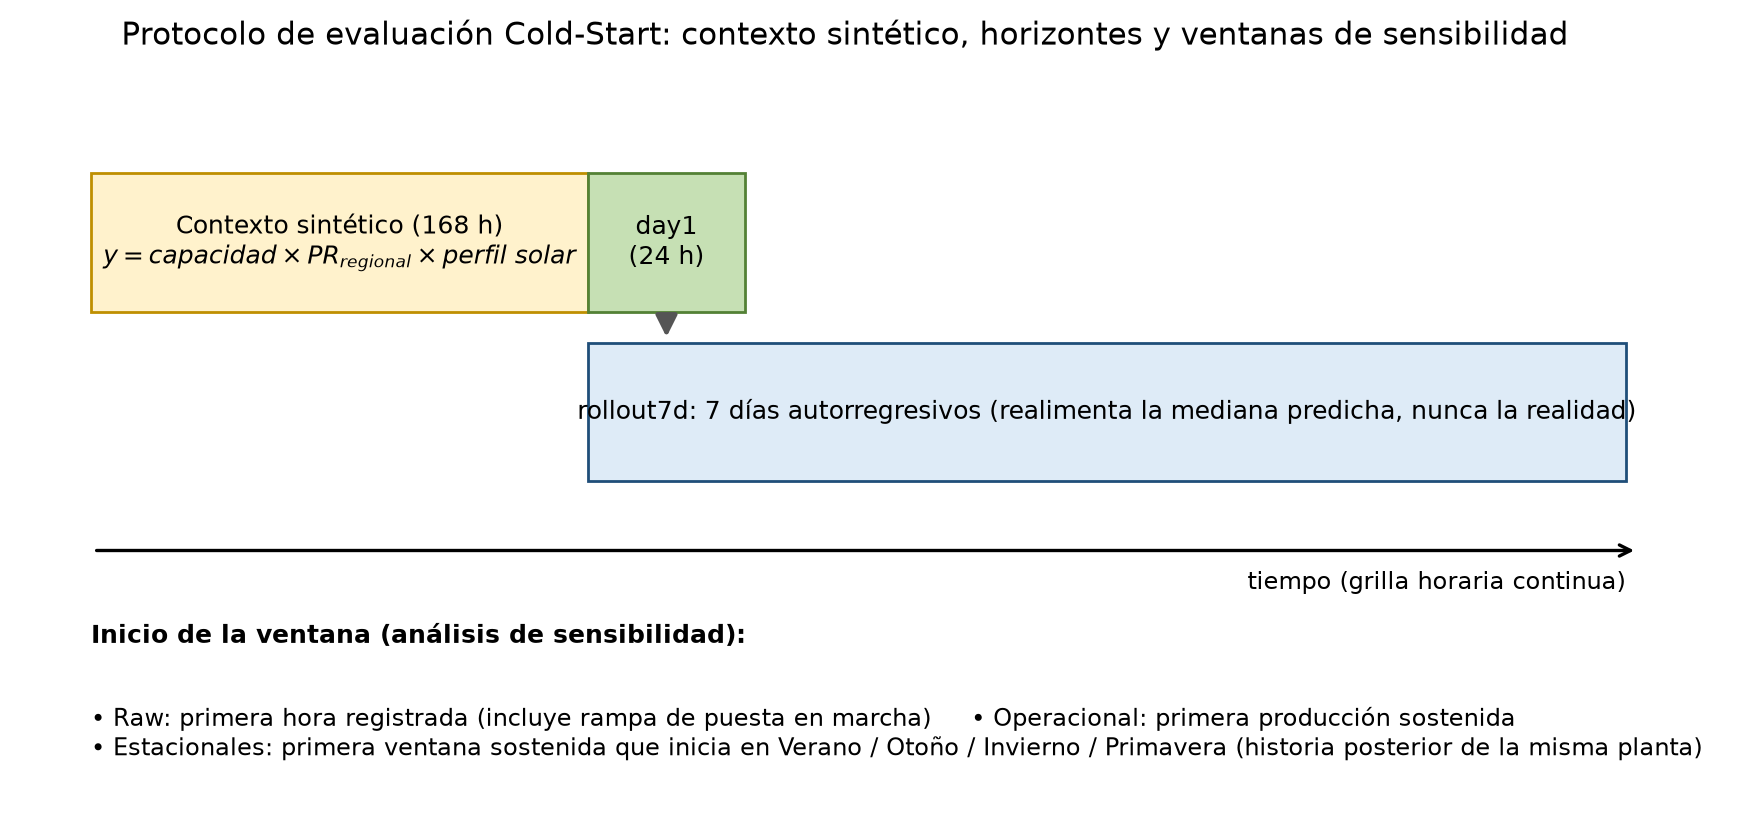
\includegraphics[width=\textwidth]{figuras/fig_eval_protocolo.png}
  \caption{\label{fig:metrics_visual} Protocolo de evaluación Cold-Start: contexto sintético, horizontes de pronóstico y ventanas del análisis de sensibilidad sobre las cuales se computan las métricas comparativas.}
\end{figure}

El cronograma temporal que ordena la ejecución de estas cuatro fases corresponde a la carta Gantt de seis semanas presentada en la Figura \ref{fig:gantt_planificacion} del Capítulo I, cuyas actividades se encuentran categorizadas según el objetivo específico al que tributan.

\subsection{Arquitectura de Componentes y Stack Tecnológico}
Más allá del flujo lógico de datos descrito en las fases anteriores, la solución se materializa como un sistema de software modular gobernado por un \textbf{orquestador único} (\texttt{src/orchestrator.py}), que constituye el único punto de entrada de producción y coordina la ejecución secuencial de las capas del \textit{pipeline}. La Figura \ref{fig:arquitectura} presenta el diagrama de componentes, la estructura de módulos y el \textit{stack} tecnológico sobre el que se implementa cada etapa.

La primera capa, \textbf{ETL} (\texttt{src/etl/}), materializa el flujo Medallion: los módulos \texttt{landing\_\allowbreak to\_\allowbreak bronze} ingieren y normalizan los archivos crudos de generación y meteorología, \texttt{bronze\_\allowbreak to\_\allowbreak silver} aplica el agrupamiento por macrozona, las variables cíclicas y la imputación auditada de exógenas, y \texttt{silver\_\allowbreak to\_\allowbreak gold\_\allowbreak split} particiona los conjuntos de prueba por planta; el módulo \texttt{prepare\_\allowbreak dl\_\allowbreak dataset} deriva la versión numérica del conjunto apta para las redes profundas. La segunda capa, \textbf{ML} (\texttt{src/\allowbreak ml/\allowbreak orchestrator\_\allowbreak ml.py}), ejecuta el bucle \textit{Leave-One-Plant-Out}: para cada planta objetivo entrena y evalúa las cinco arquitecturas globales sobre las $N-1$ plantas restantes (con el ciclo \textit{tune}$\rightarrow$\textit{train}$\rightarrow$\textit{test}) y, en paralelo, las tres líneas base estrictamente locales. La tercera capa, \textbf{Reporte}, consolida las métricas y genera las figuras y tablas del presente documento. Las tres capas se apoyan en un conjunto de \textbf{utilidades compartidas} (\texttt{src/\allowbreak ml/\allowbreak utils/}) que centralizan la lógica sensible a la integridad científica —el particionado LOPO (\texttt{data\_\allowbreak loader}), la grilla horaria canónica (\texttt{grid}), la definición de ventanas (\texttt{eval\_\allowbreak window}), el \textit{prior} regional (\texttt{regional\_\allowbreak prior}) y el cómputo de métricas (\texttt{metrics})—, evitando su duplicación y garantizando un tratamiento idéntico para todos los modelos.

El orquestador incorpora, además, dos salvaguardas de ingeniería: un \textit{gate} de pruebas automatizadas (\texttt{pytest}) que se ejecuta antes de cada corrida y detiene el \textit{pipeline} ante cualquier fallo, y un control de idempotencia mediante marcadores de completitud que permite reanudar ejecuciones largas sin recomputar trabajo ya finalizado. El \textit{stack} tecnológico se compone de Python 3.12 como lenguaje base, PyArrow/Parquet para la persistencia columnar entre capas, pandas para la manipulación tabular, el ecosistema NeuralForecast de Nixtla sobre PyTorch 2.5.1 (CUDA 12.1) para las arquitecturas profundas, XGBoost para los modelos de árboles, Optuna para la optimización de hiperparámetros y matplotlib/seaborn para la visualización.

\begin{figure}[htbp]
  \centering
  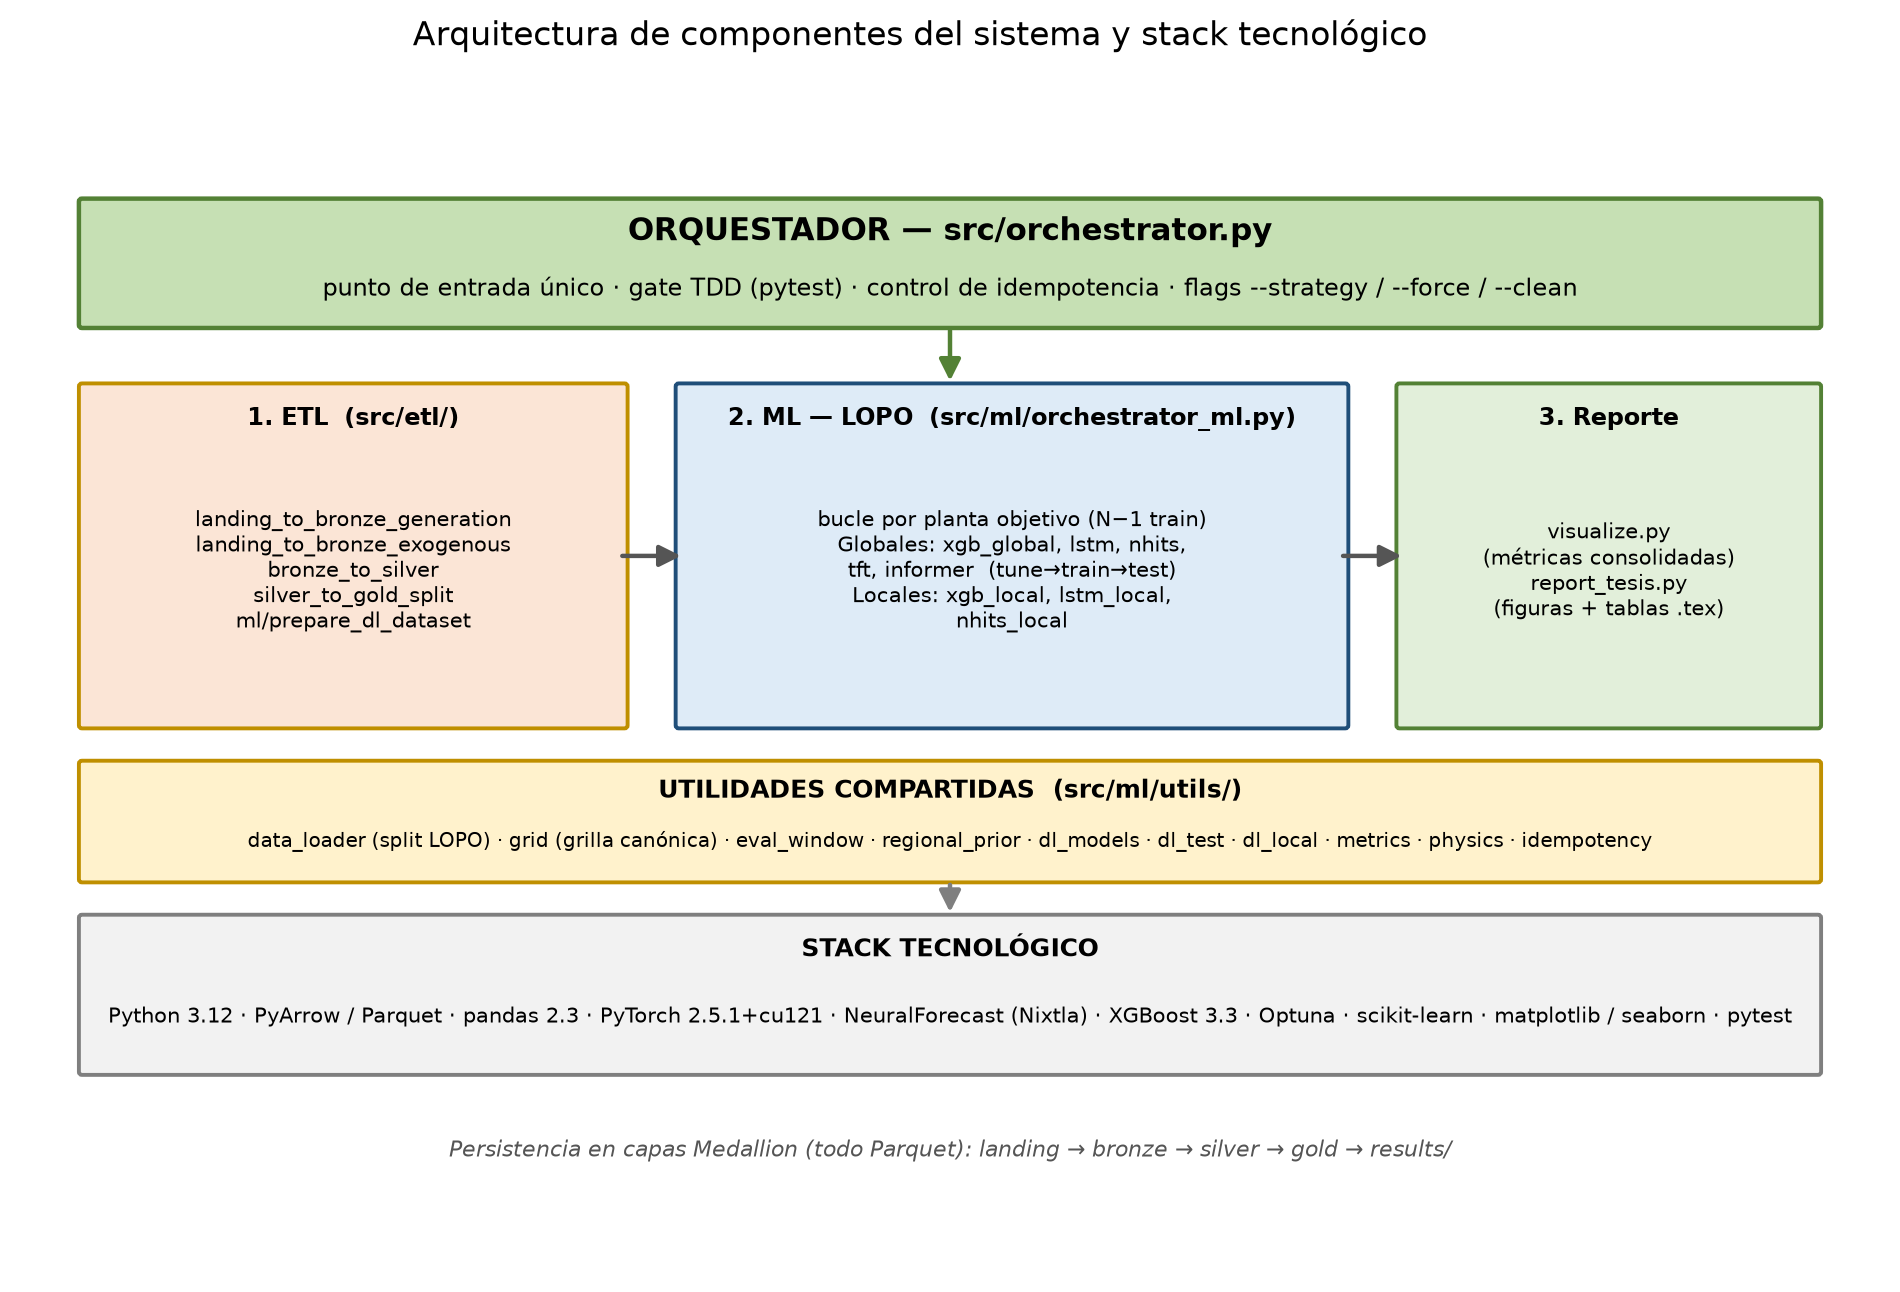
\includegraphics[width=\textwidth]{figuras/fig_arquitectura_componentes.png}
  \caption{\label{fig:arquitectura} Diagrama de componentes del sistema: orquestador único, las tres capas del \textit{pipeline} (ETL, ML--LOPO y Reporte) con sus módulos, la capa de utilidades compartidas y el \textit{stack} tecnológico que soporta cada etapa.}
\end{figure}

\FloatBarrier
\subsection{Estudio de Factibilidad}

\subsubsection{Factibilidad técnica}
La factibilidad técnica de este proyecto está garantizada por la disponibilidad de herramientas de \textit{software} de código abierto (\textit{Open Source}) y librerías especializadas en \textit{Machine Learning} y \textit{Deep Learning}. Toda la orquestación del pipeline (ETL, entrenamiento y validación) se encuentra programada en \textit{Python}, utilizando el ecosistema \textit{Nixtla} (específicamente \textit{NeuralForecast}) para la ejecución de los algoritmos atencionales de última generación (TFT y N-HiTS), así como \textit{XGBoost} para las líneas base locales. Adicionalmente, el procesamiento matricial intensivo requerido por el paradigma \textit{Cross-Site Learning} se aborda mediante el uso de aceleración por hardware computacional (GPUs), recursos que son accesibles a través de entornos de desarrollo estándar.

\subsubsection{Factibilidad operativa}
La operación del estudio es autónoma y reproducible: el pipeline completo se ejecuta desde un único punto de entrada con validación automatizada previa (gate de pruebas), control de idempotencia para reanudar corridas interrumpidas y generación automática de reportes. La extensión del análisis a nuevas plantas o períodos no requiere infraestructura ni personal adicional.

\subsubsection{Factibilidad económica}
El costo marginal del proyecto es prácticamente nulo: las fuentes de datos son públicas (Coordinador Eléctrico Nacional y red climatológica CR2), la totalidad del software empleado es de código abierto y el cómputo se resuelve en hardware de consumo (una única GPU de gama media), sin requerir financiamiento externo ni servicios de nube de pago.

\subsubsection{Factibilidad legal}
Los datos empleados provienen de repositorios públicos de organismos oficiales chilenos y no contienen datos personales ni información sujeta a confidencialidad. Las licencias de las librerías utilizadas (ecosistema Python de código abierto) son compatibles con el uso académico e investigativo del presente trabajo.

\subsubsection{Factibilidad Social}
El proyecto no genera impactos sociales adversos. Indirectamente, la mejora del pronóstico de generación en plantas recién conectadas contribuye a la estabilidad del suministro eléctrico y reduce las barreras de entrada para nuevos actores renovables de menor escala.

\subsubsection{Factibilidad Ambiental}
La investigación tributa a la descarbonización de la matriz energética al facilitar la integración temprana de nueva capacidad solar. La huella de cómputo del estudio es acotada: los entrenamientos completos se resuelven en horas sobre una única GPU, sin infraestructura de centros de datos dedicada.